\section{Тема 4} % TODO:

\subsection{Релации}
\boxt{Определение}
Нека \(n \ge 1\) и \mexpr{A_1, A_2, ..., A_n} са множество, наречена съответно първи домейн домейн, 
втори домейн, ..., \(n\)-ти домейн. Релация над декартовото произведение \mexpr{A_1 \times A_2 \times ... \times A_n}
е всяко множество \mexpr{R \subseteq A_1 \times A_2 \times ... \times A_n}.

Казваме, че \(R\) е \(n\)-местна или \(n\)-арна.

\bu{Пример за релации:} \(<, \le, >, \ge, =\) са релации над декартовия квадрат \(\mathbb{R}^2\).
Нека \(S\) е множество, \mexpr{\subseteq_{S}} е релация над \mexpr{2^S \times 2^S}, дефенирана така:
\mexpr{\forall a, b \in 2^S: (a, b) \in \subseteq_{S} \iff a \subseteq b}

Примерно, нека \mexpr{S = \{a, b\}}. Тогава \mexpr{(\{a\}, \{a, b\}) \in \subseteq_{S}, (\{a, b\}, \{a\}) \not \in \subseteq_{S}} и т.н.

\subsection{Двуместни релации над декартови квадрати и представяне чрез матрици и графи (диаграми)}
Нека \mexpr{A = \{a_1, a_2, ..., a_n\}} и \mexpr{R \subseteq A^2}.
Например, \mexpr{A = \{a, b, c, d\}, R = \{(a, a), (a, b), (c, c), (d, a)\}}. \\

\boxt{Представяне чрез матрици}

Можем да представим \(R\) чрез булева матрица \(n \times n\), в която на ред \(i\) и колона \(j\) е:
\begin{itemize}
    \item 1, ако \mexpr{a_iRa_j}
    \item 0, в противен случай
\end{itemize}

\begin{center}
    \begin{tabular}{ | c | c | c | c | c | } 
        \hline
        & a & b & c & d \\
        \hline
        a & \textcolor{red}{1} & \textcolor{red}{1} & 0 & 0 \\
        \hline
        b & 0 & 0 & 0 & 0 \\
        \hline
        c & 0 & 0 & \textcolor{red}{1} & 0 \\
        \hline
        d & \textcolor{red}{1} & 0 & 0 & 0 \\
        \hline
    \end{tabular}
\end{center}

\boxt{Представяне чрез графи} \\
Можем да представим \(R\) чрез диаграма от точки и стрелки, в която на всяко \(a_i\) съответства отделна
точка, наречена връх, а ребро от връх \(a_i\) до върха \(a_j\) има \totw \(a_iRa_j\).

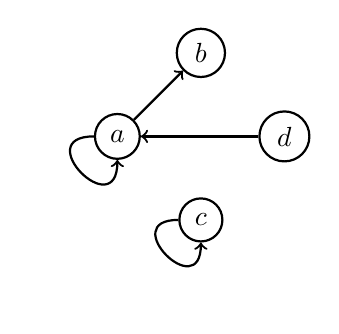
\begin{tikzpicture}[node distance={15mm}, thick, main/.style = {draw, circle}] 
    \node[main] (1) {$a$};
    \node[main] (2) [above right of=1] {$b$};
    \node[main] (3) [below right of=1] {$c$};
    \node[main] (4) [above right of=3] {$d$};
    \draw[->] (1) to [out=180,in=270,looseness=5] (1);
    \draw[->] (1) -- (2);
    \draw[->] (3) to [out=180,in=270,looseness=5] (3);
    \draw[->] (4) -- (1);
\end{tikzpicture}

\subsection{Свойства на двуместни релации}
Нека \mexpr{R \subseteq A^2}.
% TODO: left more info
\begin{enumerate}
    \item Рефлексивност \\
    \(R\) е рефлексивна \totw \mexpr{\forall a \in A: aRa}.

    \item Антирефлексивност \\
    \(R\) е антирефлексивна \totw \mexpr{\forall a \in A: \lnot aRa}.
    
    \item Симетричност \\
    \(R\) е симетрична \totw \mexpr{\forall a, b \in A, a \not = b: aRb \to bRa}.

    \item Антисиметричност \\
    \(R\) е антисиметрична \totw \mexpr{\forall a, b \in A, a \not = b: aRb \to \lnot bRa}.
    
    \item Силна антисиметричност \\
    \(R\) е силно антисиметрична \totw \mexpr{\forall a, b \in A, a \not = b: aRb \oplus bRa}.
    
    \item Транзитивност \\
    \(R\) е транзитивна \totw \mexpr{\forall a, b \in A : aRb \land bRc \to aRc}.
    
\end{enumerate}

\subsection{Затваряния на релации}
Рефлексивното/симетричното/транзитивното затваряне на \(R\) е минималното множество \mexpr{R^{'} \subseteq A^2}, 
такова че \mexpr{R \subseteq R^{'}} и \(R^{'}\) е рефлексивна/симетрична/транзитивна релация.

"\(R^{'}\) е минималното множество" означава, че за всяко \mexpr{R^{''} \subseteq A^2}, такова че 
\mexpr{R \subseteq R^{''}} и \(R^{''}\) е рефлексивна/симетрична/транзитивна, е вярно, че \mexpr{R^{'} \subseteq R^{''}}.

Релация е рефлексивна/симетрична/транзитивна \totw съвпада с рефлексивното/симетричното/транзитивното си 
затваряне.

\boxt{Допълнение} \\
Нека \(A\) е крайно и релациите над \(A\) са представени с матрици.

Рефлексивното затваряне се получава с едно сканиране на главния диагонал и обръщане на всяка \(0\) в \(1\).
Симетричното затваряне се получава чрез сканиране за двойки \((0; 1)\) и \((1; 0)\), които са симетрично
спрямо главния диагонал, и обръщане на \(0\)-та от двойката в \(1\)-ца.

\subsection{Релации на еквивалентност}
Релация е релация на еквивалентност \totw рефлексивна, симетрична и транзитивна.

\bu{Пример:} \(=\)

Нека \mexpr{R \subseteq A^2} е релация на еквивалентност. За всеки елемент \mexpr{a \in A} дефенираме
множеството \mexpr{[a] = \{b \in A | aRb\}}.

\subsection{Теорема за класовете на еквивалентност}
Фамилията \mexpr{\{[a] | a \in A\}} е разбиване на \(A\). Елемените на тази фамилия се наричат 
\bu{класове на еквивалентност}.

\begin{proof}
    $ $\newline
    \begin{itemize}
        \item Всеки елемент на \(A\) е в поне един елемент на фамилията, понеже в \mexpr{\{[a] | a \in A\}} 
        \(a\) взема последователно стойностите на всички елементи от \(A\).
        \item Всеки елемент на фамилията е непразен, понеже \(R\) е рефлексивна.
        \item Всеки два различни елемента на фамилията имат празно сечение.
        \begin{lemma}
            \mexpr{[a] \not = [b] \to [a] \cap [b] = \emptyset}
            \begin{proof}
                $ $\newline
                Контрапозитивното е \mexpr{[a] \cap [b] \not = \emptyset \to [a] = [b]}. \\
                Да допуснем, че \mexpr{[a] \cap [b] \not = \emptyset} за някои \mexpr{a, b \in A}. \\
                Щом \mexpr{[a] \cap [b] \not = \emptyset}, то \mexpr{\exists c \in A: c \in [a] \cap [b]}. \\
                Да разгледаме елемент \mexpr{d \in [a]}. Визуално: \\
                Знаем, че \mexpr{a \in [a]} и \mexpr{b \in [b]}. \\
                От допускането имаме, че \mexpr{(1)(c \in [a] \implies aRc)} и \mexpr{(2)(c \in [b] \implies bRc)}. \\
                По дефиниция \mexpr{[a] = \{x \in A | aRx\}}. \\
                Тогава: \\
                \mexpr{aRd \to dRa} (симетричност) \\
                \mexpr{dRa \land aRc \to dRc} (транзитивност) \\
                \mexpr{cRb} (симетричност и (2)) \\
                \mexpr{dRc \land cRb \to dRb} (транзитивност) \\
                \mexpr{dRb \implies bRd} (симетричност) \\
                \mexpr{bRd \implies d \in [b]} \\
                Доказахме, че \mexpr{d \in [a] \to d \in [b]} за произволен елемент \(d\). \\
                Следователно \mexpr{[a] \subseteq [b]}. \\
                Аналогично доказваме, че \mexpr{[b] \subseteq [a]} и от аксиомата за обема получаваме, че
                \mexpr{[a] = [b]}.
            \end{proof}
        \end{lemma}
    \end{itemize}
\end{proof}